% !TeX spellcheck = en_GB
% !TeX program = pdflatex
%
% LuxSleek-CV 1.1 LaTeX template
% Author: Andreï V. Kostyrka, University of Luxembourg
%
% 1.1: added tracking and letter-spacing for prettier lower caps, added `~` for language levels
% 1.0: initial release
%
% This template fills the gap in the available variety of templates
% by proposing something that is not a custom class, not using any
% hard-coded settings deeply hidden in style files, and provides
% a handful of custom command definitions that are as transparent as it gets.
% Developed at the University of Luxembourg.
%
% *NOTHING IS HARCODED, and never should be.*
%
% Target audience: applicants in the IT industry, or business in general
%
% The main strength of this template is, it explicitly showcases how
% to break the flow of text to achieve the most flexible right alignment
% of dates for multiple configurations.

\documentclass[11pt, a4paper]{article} 

\usepackage{fontawesome} % Font Awesome for using icons
\usepackage{enumitem}  % For controlling list indentation and spacing
\usepackage{anysize}   % For customizing margins if needed

\usepackage[T1]{fontenc}     % We are using pdfLaTeX,
\usepackage[utf8]{inputenc}  % hence this preparation
\usepackage[british]{babel}  
\usepackage[left = 0mm, right = 0mm, top = 0mm, bottom = 0mm]{geometry}
\usepackage[stretch = 25, shrink = 25, tracking=true, letterspace=30]{microtype}  
\usepackage{graphicx}        % To insert pictures
\usepackage{xcolor}          % To add colour to the document
\usepackage{marvosym}        % Provides icons for the contact details

\usepackage{enumitem}        % To redefine spacing in lists
\setlist{parsep = 0pt, topsep = 0pt, partopsep = 1pt, itemsep = 1pt, leftmargin = 6mm}

\usepackage{FiraSans}        % Change this to use any font, but keep it simple
\renewcommand{\familydefault}{\sfdefault}

\definecolor{cvblue}{HTML}{304263}

%%%%%%% USER COMMAND DEFINITIONS %%%%%%%%%%%%%%%%%%%%%%%%%%%
% These are the real workhorses of this template
\newcommand{\dates}[1]{\hfill\mbox{\textbf{#1}}} % Bold stuff that doesn’t got broken into lines
\newcommand{\is}{\par\vskip.5ex plus .4ex} % Item spacing
\newcommand{\smaller}[1]{{\small$\diamond$\ #1}}
\newcommand{\headleft}[1]{\vspace*{3ex}\textsc{\textbf{#1}}\par%
    \vspace*{-1.5ex}\hrulefill\par\vspace*{0.7ex}}
\newcommand{\headright}[1]{\vspace*{2.5ex}\textsc{\Large\color{cvblue}#1}\par%
     \vspace*{-2ex}{\color{cvblue}\hrulefill}\par}
%%%%%%%%%%%%%%%%%%%%%%%%%%%%%%%%%%%%%%%%%%%%%%%%%%%%%%%%%%%%

\usepackage[colorlinks = true, urlcolor = white, linkcolor = white]{hyperref}

\begin{document}
% Style definitions -- killing the unnecessary space and adding the skips explicitly
\setlength{\topskip}{0pt}
\setlength{\parindent}{0pt}
\setlength{\parskip}{0pt}
\setlength{\fboxsep}{0pt}
\pagestyle{empty}
\raggedbottom
\begin{minipage}[t]{0.33\textwidth} %% Left column -- outer definition
%  Left column -- top dark rectangle
\colorbox{cvblue}{\begin{minipage}[t][5mm][t]{\textwidth}\null\hfill\null\end{minipage}}

%\vspace{-.2ex} % Eliminates the small gap
\colorbox{cvblue!90}{\color{white}  %% LEFT BOX
\kern0.09\textwidth\relax% Left margin provided explicitly
\begin{minipage}[t][293mm][t]{0.82\textwidth}
\raggedright
\vspace*{2.5ex}

\Large Shariff Bukhary bin Sharifuzan \normalsize 

% Centering without extra vertical spacing
\null\hfill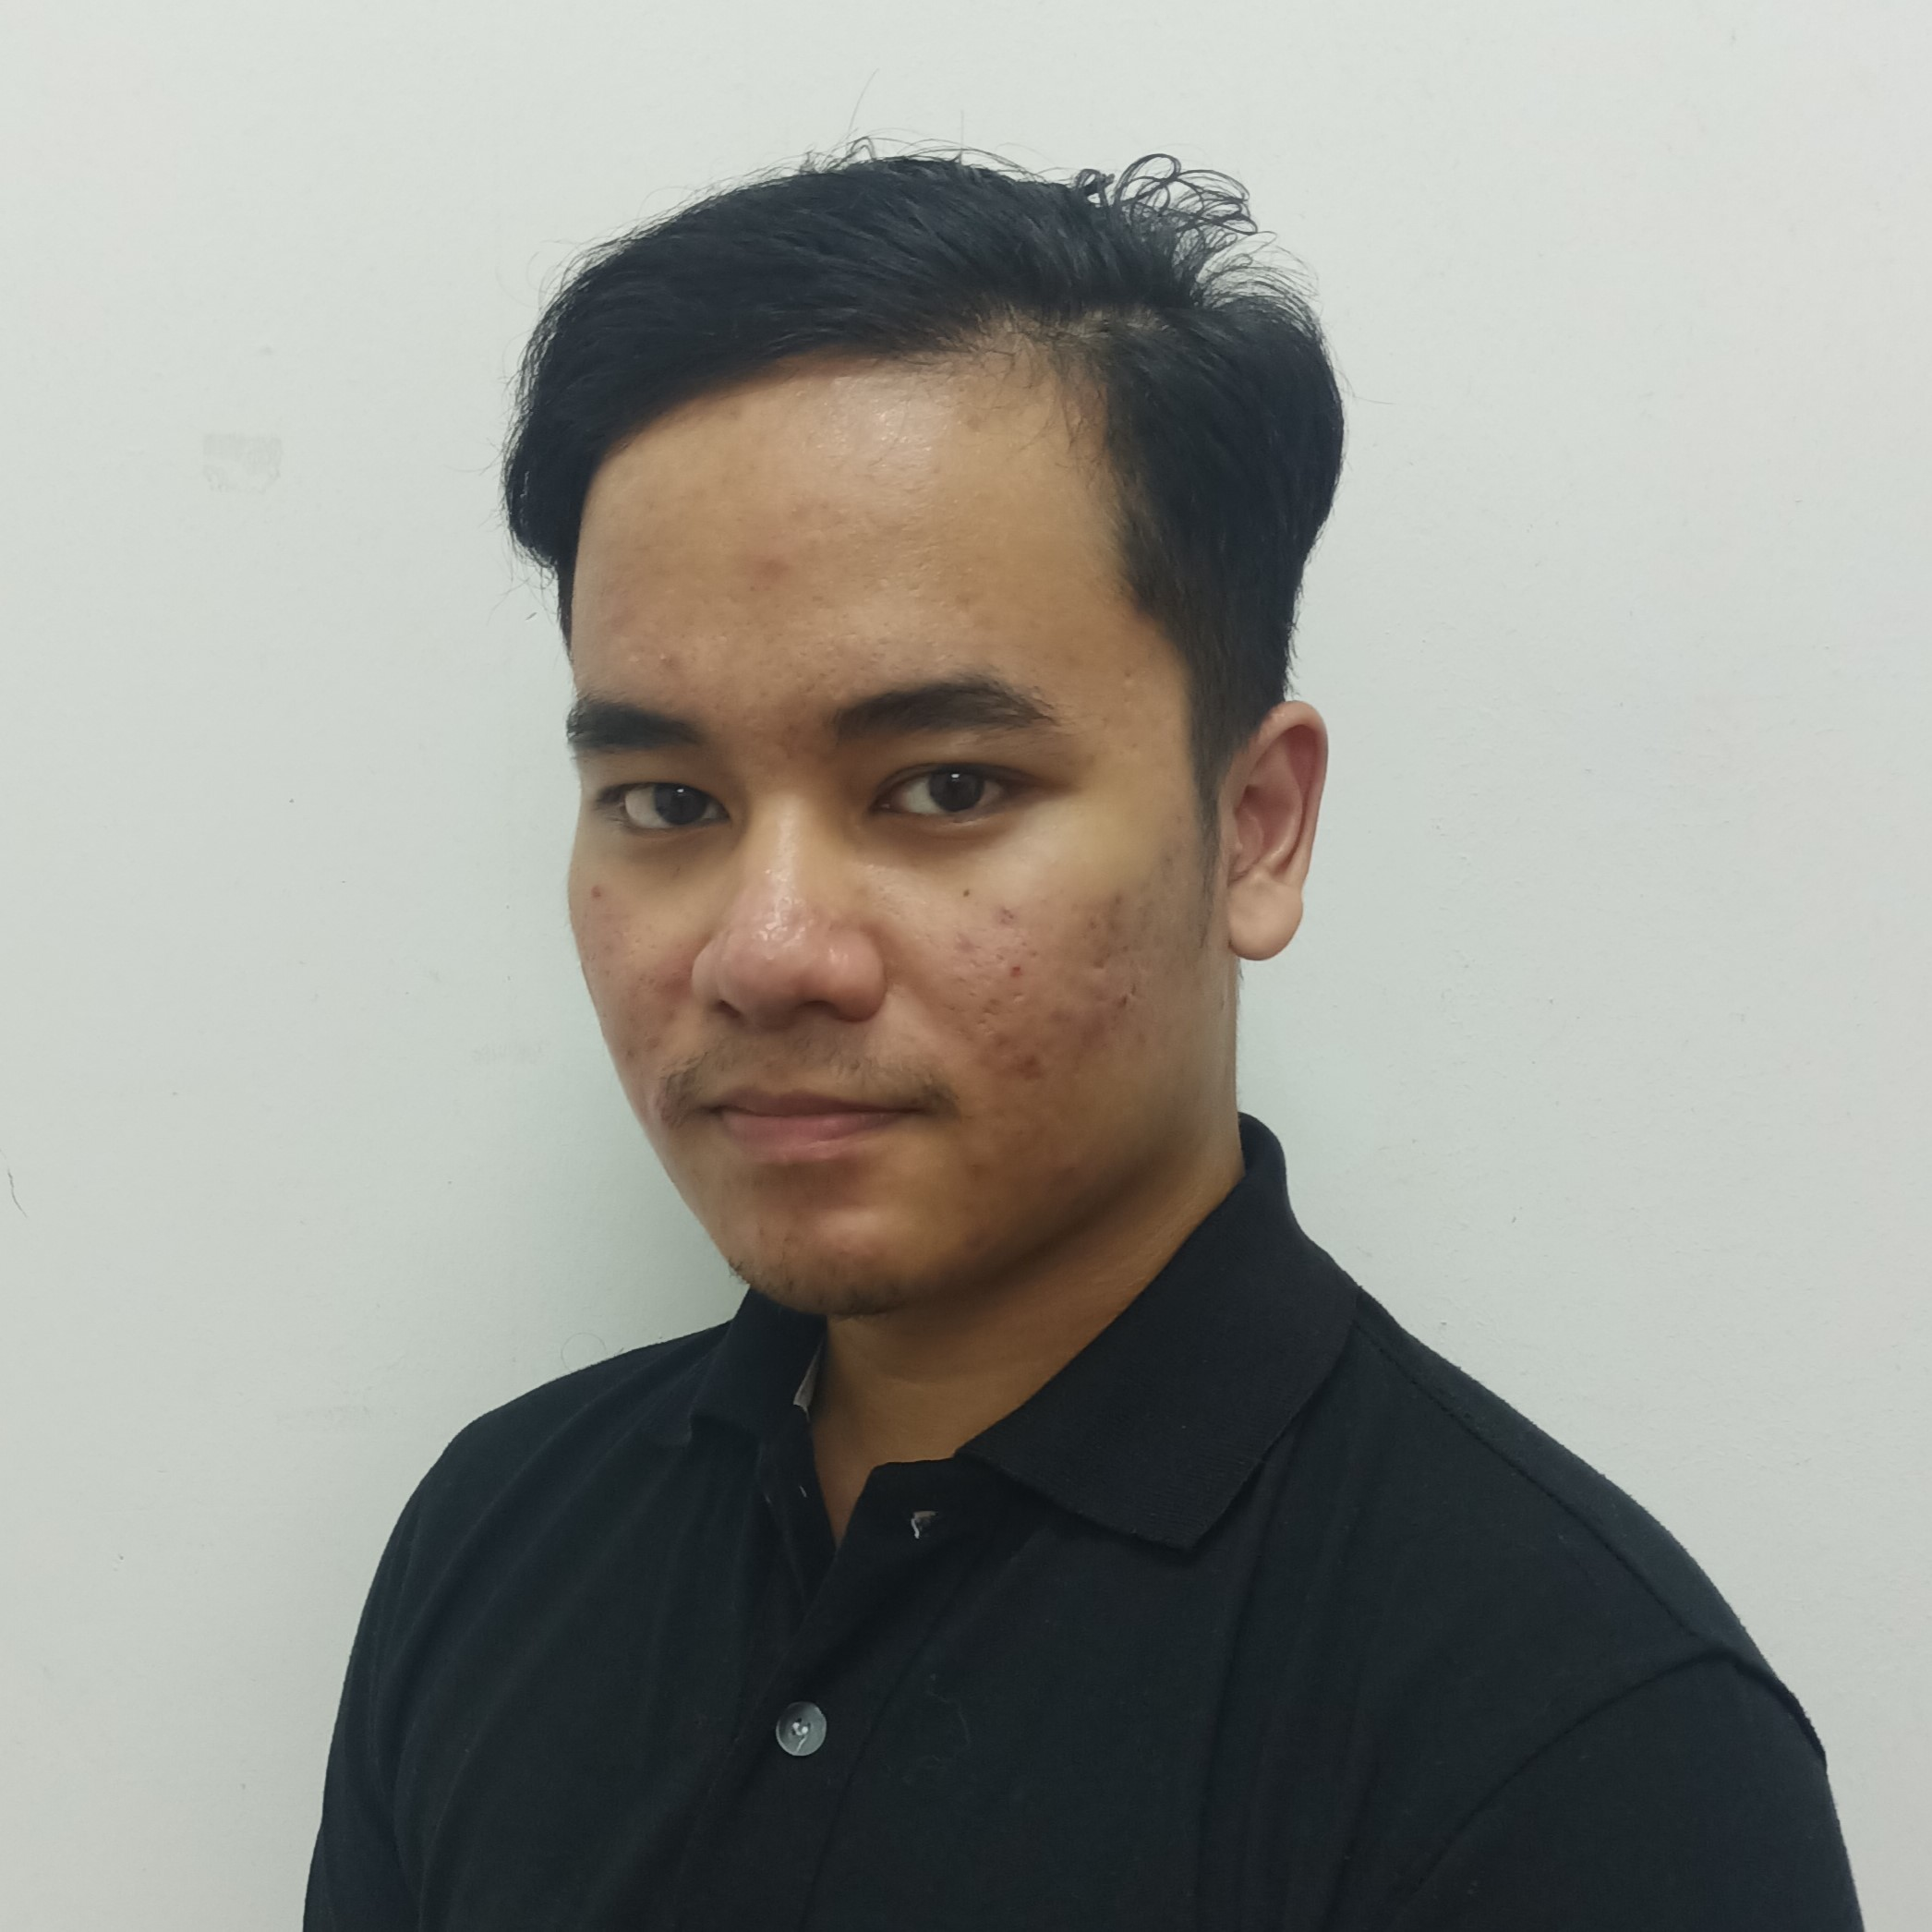
\includegraphics[width=0.65\textwidth]{side-pic-square.jpg}\hfill\null

\vspace*{0.5ex} % Extra space after the picture

\headleft{Career Objective}
Motivated recent graduate with extensive experience in handling software
and programming languages to provide functional and robust software
solutions, seeking to reinforce and expand \textit{back-end development} skills
and knowledge pool.

\headleft{Contact details}
\small % To fit more content
\MVAt\ {\small shariffbukhary01@gmail.com} \\[0.4ex]
\Mobilefone\ +60\,11\,6984\,1369\\[0.5ex]
\Letter\ 319, Jalan Bukit Citra 4/5,
Taman Bukit Citra,
71700 Mantin, N. Sembilan
\normalsize

\headleft{Technical Skills}
\textbf{Programming Languages}
\begin{itemize}
\item JavaScript (server-side)
\item Python
\item HTML/CSS
\end{itemize}

\vspace{0.2cm}

\textbf{Web Frameworks}
\begin{itemize}
\item Express.js
\item Flask
\item Streamlit
\end{itemize}

\vspace{0.2cm}

\textbf{Databases Initialization and Queries}
\begin{itemize}
\item MySQL (Sequelize)
\item MongoDB (Mongoose.js)
\item SQLite (SQLAlchemy)
\end{itemize}

\end{minipage}%
\kern0.09\textwidth\relax%%Right margin provided explicitly to stretch the colourbox
}
\end{minipage}% Right column
\hskip2.5em% Left margin for the white area
\begin{minipage}[t]{0.56\textwidth}
\setlength{\parskip}{0.8ex}% Adds spaces between paragraphs; use \\ to add new lines without this space. Shrink this amount to fit more data vertically

\vspace{2ex}

\headright{Work Experience}

\textsc{Library Management System} at \textit{TalentLabs Academy.}  \dates{2024.08} \\

\smaller{Developed a library management system using Express.js and
JavaScript for easier book-borrowing management.}

\is
\smaller{Configured role-based access with Passport.js to segregate
and protect sensitive data from unauthorized access from a
normal user and relegates the critical data to system admins.}

\is
\smaller{Provided abstraction layers by defining separate functions in separate classes and files for improved code readability and easier debugging.}

\vspace
\textsc{Contact Manager Project} at \textit{TalentLabs Academy.}  \dates{2024.09} \\

\is
\smaller{Designed and constructed a backend system for contact management using Express.js for a quicker and more lightweight experience in creating, modifying, and deleting contacts.}

\is
\smaller{Enabled partitioning of the contacts according to registered and logged in user details, utilizing JSON web tokens (JWT) and MongoDB to provide scalable and sustainable solutions for assigning contacts to the corresponding users.}

\is 
\smaller{Improved user privacy protection by introducing private routing for sensitive information and using Bcrypt for salting and hashing private info before saving to MongoDB, ensuring user data security and safety in the case of a data breach.}

\vspace
\textsc{Project SHARIF (Smart and Handy Automated Rotating Intelligent Fan) (Arduino)} at \textit{International Islamic University of Malaysia.}  \dates{2024.07} \\

\is
\smaller{Collaborated with a team of 3 people in developing a climate
control device with Arduino to achieve fully automated
ambient temperature control.} 

\is
\smaller{Programmed and deployed an algorithm for controlling the
functions and parameters of the climate control device such as
ambient temperature and wind flow speed to enable remote and automated functioning of the device.}

\is
\smaller{Having good knowledge creating Relationships in data model like one-one, one-many, many-one and many-many. Monitoring and validating key metrics insights data from daily report.}

\headright{Education}

\textsc{Back-End Development Trainee.} \textit{from TalentLabs Academy}. \dates{2024.09--2024.12} \\

\is
\textsc{Bachelor of Science (Physics) (Hons).} \textit{from International Islamic University of Malaysia}.  \dates{2021--2024} \\

\end{minipage}

\end{document}
